\documentclass[main.tex]{subfiles}
\begin{document}
    \section{Embedded}
    \subsection{Microcontroller}
    \subsection{Custom Software}
    \subsection{Buses}
    \subsection{Main Embedded Board}
    Raspberry Pi’s will be socketed on the main embedded board face down (as described by the CAD). Due to the complexity of the board, and minimal space saved by integrating the board onto the main embedded system, the Pi will not be integrated directly onto the main embedded. Furthermore, in case of a malfunction it is more cost and time effective to replace a singular Pi instead of replacing the entire board. The Arduino Mega will be integrated directly onto the board. Since once complete the Arduinos will not have to be frequently updated, it would be efficient to simply use a ATmega 328, DIP-28 package and pop it out to program it on a regular Mega board when necessary. The choice for a DIP package over a TQFP was also made such that a blown chip would not lead to the entire board having to be replaced.

    \subsection{Subsystem Boards}
    Originally, the embedded team decided to use an Arduino Uno, with a CANBUS shield stacked on top, with a seperate board with the connections to the external connectors on it. However, most of the pins on both the arduino and the CANBUS were completely unnecessary. With said design, the embedded for a single subsystem would be almost triple the size of an Arduino Uno, with significantly more sources of error (the Arduino, the CANBUS, and a board housing connectors would have to be connected together).  Upon considering that there would have to be multiple of these housings, it was decided that all three boards could be integrated into a singular one, with the approximate size of an Arduino Uno. Once the final revision is designed, multiple copies of the same board will be printed and populated. For initially testing purposes however the original setup of an Uno with a CANBUS shield will be used, until the PCB is printed and thoroughly tested.

    \subsection{Sensors}
    \subsubsection{Temperature}
    \subsubsection{Current}
    \subsubsection{Tilt}
    \subsubsection{Navigation}
    \subsubsection{Lateral Stability}
    \subsubsection{EC-Brake State}
    \subsubsection{Pressure}

    \subsection{Thermal}
    \subsection{Flowcharts}

    \subsection{Physical Hardware}
    Mass, power, etc.\\
    How will these things be powered? Mini lipo battery packs?\\
    How is it mounted? CAD? Does it need to be in a pressure chamber?\\
    Will the processors get very hot due to vacuum? How will they be cooled?\\
    Will the system have components susceptible to vacuum? (e.g. some capacitors) Briefly justify an answer of “no.” How will we test this?\\
    Rationale for choosing Raspberry Pi and Arduino\\
    Cost breakdown

    \subsection{Software System Structure}
    \subsubsection{Terminology}
    \begin{itemize}
        \item Control-Panel - UI interface running on a remote machine to visualize data and control pod
        \item Master Machine - RaspberryPi 3B computer running Waterloop’s communication-system
        \item Slave Machine - Arduino Due running Waterloop’s embedded-system
        \item CAN Data Packet - Custom binary packet type created by team Waterloop
    \end{itemize}
    \subsubsection{Design Criteria}
    The main goal  when building the software systems around the pod was creating a redundant, yet lightweight and fast solution that would allow for safe communications with the vehicle and ensure control throughout pod launch. The Software-system is built upon the Master-Slave design model to allow for maximum redundancy and safety at all times. The design is based on three components: embedded systems (Slave), communication systems (Master), and control-panel. Embedded-systems is responsible for all of the pod’s internal interactions with the sensors and various health checks. Communication-systems is responsible for the complete pod control and has the ability to safely shut down the pod in case of an emergency. It is also responsible for the transportation of information from the vehicle to the front-end to allow for live data visualization and remote control of the pod. Front-end is responsible for displaying all of the pod’s vital readings and providing an interface to control the pod while in the tube. All of the code written for the software system of the pod is available for public access at Waterloop’s github page.
    \subsubsection{System Overview}
    Building off the model of Master-Slave design, Waterloop has defined two clear computational layers Master Machines and Slave Machines. Master machines are responsible for the complete control of the pod and the transfer of data from Slave Machines to the Control-Panel. Two main design decisions of the Goose III’s computational design are the parallelism of launch script execution and the Master-slave design.
    \begin{itemize}
        \item Having Master-Slave design in place, we can ensure the validity of data coming from the Slave Machines. When Slaves acquire data from sensors, there is a possibility of a slave providing errant data. To handle the case of an errant slave, Masters have the voting capability to compare the results of three slaves, detect the errant device and act appropriately
        \item With parallel execution by the two Master machines, in case of one of the machines coming offline for any unforeseen reason, the switch to the next machine is instantaneous
    \end{itemize}
    \textbf{[INSERT SOFTWARE DIAGRAM HERE]}\\
    Based on the software diagram above, the entire system will incorporate \textbf{[Number of sensors]} sensors and an ESC, that will allow for a complete control over the pod and a live stream of data from all sensors.
    \subsection{Control Packet Format}
    \subsubsection{JSON}
    All communications between onboard computers and frontend controls are JSON packets serialized from Go structs in the following format:
    \begin{verbatim}
type CommPacketJson struct {
    Time int64     `json:"time"`
    Type string    `json:"type"`
    Name string    `json:"name"`
    Data []float32 `json:"data"`
}
    \end{verbatim}
    \begin{table}[H]
        \centering
        \begin{tabularx}{\textwidth}{@{}lXl@{}} \toprule
            Property & Description & Example\\ \midrule
            \verb|time| & Time of packet creation, in milliseconds since Unix epoch & \verb|1513452619442|\\
            \verb|type| & Packet type, see possible packet types & \verb|"sensor"|\\
            \verb|name| & Specific name of packet, explicitly describing role and origin of packet (i.e. data from a specific sensor) & \verb|"accel1"|\\
            \verb|data| & 3-tuple of float32 values representing packet data & \verb|[32.2323, 12.22, 23.11]|\\ \bottomrule
        \end{tabularx}
        \caption{Explanation of fields}
    \end{table}
    Example of a serialized JSON:
    \begin{verbatim}
{
    "time": 1513452619442,
    "type": "sensor",
    "name": "accel",
    "data": [0.00, 0.00, 0.00]
}
    \end{verbatim}
    \subsubsection{Binary Packet Structure}
    Communication between slaves (Arduino) and onboard masters (Raspberry Pi) consist of 8 byte CAN data packets that are analogous to its JSON counterparts described in the previous section.
    \begin{table}[H]
        \centering
        \begin{tabularx}{\textwidth}{@{}XXXXX@{}} \toprule
            {[0:2]} & {[3:9]} & {[10:27]} & {[28:45]} & {[46:63]}\\ \midrule
            000 & 0000000 & 000000000000000000 & 000000000000000000 & 000000000000000000\\
            Packet Type & Packet Name & Data value 1 & Data value 2 & Data value 3\\
            Packet type, see below & Packet name, of 127 possible names & Sensor Data location 1 & Sensor Data Location 2 & Sensor Data location 3 \\ \bottomrule
        \end{tabularx}
        \caption{Caption needed}
    \end{table}
    \paragraph{Packet Type Representation}
    Each packet type is represented by 3 bit encoding
    \begin{table}[H]
        \centering
        \begin{tabular}{@{}ll@{}} \toprule
            Bits & Type\\ \midrule
            000 & sensor\\
            001 & command\\
            010 & state\\
            011 & log\\ \bottomrule
        \end{tabular}
        \caption{Caption needed}
    \end{table}

    \paragraph{Packet Name Representation}
    Each packet name is represented by 7 bits.\\
    \textbf{To be determined}
    \begin{table}[H]
        \centering
        \begin{tabular}{@{}ll@{}} \toprule
            Bits & Name\\ \midrule
            0000000 & start\\
            0000001 & sensor1\\
            0000010 & sensor2\\ \bottomrule
        \end{tabular}
        \caption{Caption needed}
    \end{table}

    \paragraph{Data representation}
    Data values are floats represented by 18 bits as follows:
    \begin{table}[H]
        \centering
        \begin{tabular}{@{}lll@{}} \toprule
            Sign & Exponent & Significand\\ \midrule
            1 bit & 5 bits & 12 bits\\ \bottomrule
        \end{tabular}
        \caption{Caption needed}
    \end{table}
    This allows us a max value of \verb|65504| and a minimum positive normal of about \verb|1.5258789e-5| with approximately 4 significant digits.
    \subsection{Communication Packet Types and Usage}
    Packets can be exchanged between embedded systems, onboard controllers and frontend controls depending on type.
    \subsubsection{Command}
    Command packets are unidirectional from frontend controls to the pod.
    \begin{table}[H]
        \centering
        \begin{tabularx}{\textwidth}{@{}lllX@{}} \toprule
            Name & Code & Value(s) & Example\\ \midrule
            Brake & \texttt{brk} & None & \texttt{\{"time": ..., "type": "command", "name": "brk", "data": []\}}\\
            Emergency & \texttt{emg} & None & \texttt{\{"time": ..., "type": "command", "name": "emg", "data": []\}}\\
            Speed & \texttt{spd} & \texttt{0.00 - 100.00} & \texttt{\{"time": ..., "type": "command", "name": "spd", "data": [100.00]\}}\\
            Start Pod & \texttt{start} & None & \texttt{\{"time": ..., "type": "command", "name": "start", "data": []\}}\\
            Stop Pod & \texttt{stop} & None & \texttt{\{"time": ..., "type": "command", "name": "stop", "data": []\}}\\
            Health Check & \texttt{health} & None & \texttt{\{"time": ..., "type": "command", "name": "health", "data": []\}}\\
            Coast & \texttt{coast} & None & \texttt{\{"time": ..., "type": "command", "name": "coast", "data": []\}}\\
            Accelerate & \texttt{accel} & None & \texttt{\{"time": ..., "type": "command", "name": "accel", "data": []\}}\\ \bottomrule
        \end{tabularx}
        \caption{Caption needed}
    \end{table}

    \subsubsection{Sensor}
    Sensor packets are unidirectional from pod sensors to controllers and frontend. \textbf{Unfinished, update with actual sensors}
    \begin{table}[H]
        \centering
        \begin{tabularx}{\textwidth}{@{}lllX@{}} \toprule
            Name & Code & Value(s) & Example \\ \midrule
            {[Sensor Name]} & \texttt{[sensor code]} & None & \texttt{\{"time": ..., "type": "sensor", "name": "accel", "data": [12.11, 12.34, 43.21]\}} \\ \bottomrule
        \end{tabularx}
        \caption{Caption needed}
    \end{table}

    \subsubsection{Log}
    Events triggering controllers to write data to log
    \begin{table}[H]
        \centering
        \begin{tabularx}{\textwidth}{@{}lllX@{}} \toprule
            Name & Code & Value(s) & Example \\ \midrule
            {[Any name]} & \texttt{[any code]} & Any values & \texttt{\{"time": ..., "type": "log", "name": "accel", "data": [12.11, 12.34, 43.21]\}} \\ \bottomrule
        \end{tabularx}
        \caption{Caption needed}
    \end{table}
    \subsubsection{State}
    Sent from embedded systems to update controllers and frontend of updates to pod state
    \begin{table}[H]
        \centering
        \begin{tabularx}{\textwidth}{@{}lllX@{}} \toprule
            Name & Code & Value(s) & Example \\ \midrule
            Speed & \texttt{spd} & \texttt{0.00 - 100.00} & \texttt{\{"time": ..., "type": "state", "name": "spd", "data": [12.11]\}} \\
            Braking & \texttt{brk} & \texttt{0, 1} & \texttt{\{"time": ..., "type": "state", "name": "brk", "data": [1]\}} \\ \bottomrule
        \end{tabularx}
        \caption{Caption needed}
    \end{table}
    \subsection{Server and Network Protocols}
    \subsubsection{Golang Server}
    Go allows for language level concurrency with Go routines and has faster raw performance than our previous event-based Node.js server, decreasing overall latency. The server acts as a middle communication channel between the low level arduino sensors and the high level frontend and executes commands from the front end.
    \subsubsection{CANBUS}
    Raw data will be transmitted through the CAN bus for communication between low level arduino sensors and the communication server.
    \paragraph{CANBUS Protocol Description}
    **TODO add more details
    \subsubsection{QUIC Streams}
    QUIC has built-in data reliability checks to eliminate packet loss and establishes connections much faster than TCP by removing the slow handshake process. It is built on top of UDP and allows for multiplexing to provide extremely fast data transmission rates with minimal latency.\\
    After testing packet transmission speeds over a fairly stable wireless connection using TCP, UDP and QUIC streams, results showed that multiplexed QUIC significantly outperformed both TCP and reliable UDP. QUIC was able to send approximately 100 data packets per millisecond whereas TCP and UDP hovered around 10 to 15 data packets per millisecond.\\
    QUIC streams will be used to transmit raw data wirelessly to the central communications controllers and the high level front end client and to transmit commands from the client to the controllers.\\
    Multiple input and output streams can be opened across the server and client which allows for the simultaneous transmission of data packets from different sensors. Individual ordered output streams will be used for important sensor data packets that require ordered processing. The input streams listen to the client for comms packets.
    \subsection{Distributed Controller Architecture}
    Todo: independent stateless masters with heartbeat + command/sensor verification on client side?
    \subsubsection{Raspberry Pi Docker Swarm}
    High levels of fault tolerance and redundancy will be achieved by running three Raspberry Pi controllers at the same time using a Docker Swarm. This will use the Raft consensus algorithm with an internal distributed state store to determine validity of data for each node and verify consistent data across all three controllers. The nodes will communicate through ethernet/HTTP Protocols.\\
    The Docker Swarm allows for two types of nodes, the manager node and worker node. Manager nodes distribute tasks among other worker nodes, and send data to the client through the communications protocols described above. Worker nodes perform the same tasks as other workers to reach consensus and can have tasks distributed among them.\\
    Initially at runtime, the pod will have a single manager node and two worker nodes running concurrently, where in the case of a manager failure, one of the worker nodes will be promoted to a manager.\\
    Controller failure will be monitored through a heartbeat managed by Docker which uses a small timeout for nodes to respond.
    \subsubsection{Data Logging and Blackbox}
    In the short-term, Generic data logging will be implemented by storing all transmitted sensor data and pod commands into JSON files onto the Raspberry Pi as a blackbox. Data from each sensor will be written to separate files to allow for future data processing and analysis of patterns.\\
    As a long-term data storage solution, Waterloop will use AWS S3 to store large amounts of data without sacrificing accesibility. For post-launch data analytics, a local Grafana UI will be built to provide quick and modular data visualization tools, thus allowing the team to debug every single test pod launch.
    \begin{itemize}
        \item CAN Bus / I2C
        \item Data machines, Controllers, etc.
        \item Any distributed systems - Master-slave vs swarm
        \begin{itemize}
            \item Protections and failovers
            \item How will we make sure there are no strange inter-device interactions that delay braking?
            \begin{itemize}
                \item Reasoning for why multiple raspberry pis is in fact better, and not simply making things overly complex
            \end{itemize}
            \item How will we make sure the real-time system is working exactly deterministically as expected?
            \item How will we test the accuracy of the navigation system?
        \end{itemize}
        \item Communication protocols
        \item Failure scenarios and state diagram
        \item List of dashboard commands
        \item Implementation of the Pod-Stop command
        \item Data logging
    \end{itemize}

    \subsection{Communication Protocol}
    Commands, sensor data, and events are sent between data machines, controllers, and web servers, using 64-bit packets. Packets are memory-		efficient, fast to read and write, and reliable. Packets are checked with a CRC-8 checksum $(0$x$97 = x^8 + x^5 + x^3 + x^2 + 1)$.
    \begin{table}[H]
    	\centering
    	\begin{tabular}{@{}lccccc@{}} \toprule
            Segment & Type & Sensor ID & Data 1 & Data 2 & Data 3 \\ \midrule
            Bits & 3 & 7 & 18 & 18 & 18 \\ \bottomrule
        \end{tabular}
        \caption{Caption here}
    \end{table}
    Each packet contains 3 bits representing packet type, 7 bits representing origin sensor or device ID, and three 18-bit data segments. These are 18-bit floats with 1 bit for sign, 5-bit exponent width, and 13-bit significand precision (12 explicitly stored), similar to IEEE 754 specifications.
	\begin{figure}[H]
        \centering
        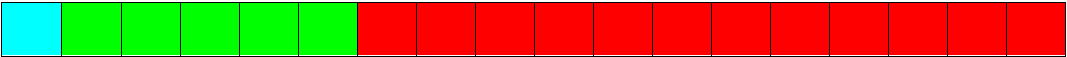
\includegraphics[width = \textwidth]{images/fig326}
    	\caption{Caption here}
    \end{figure}
    \subsection{Navigation System}
    \begin{itemize}
        \item State machine [important! Refer to MIT’s, theirs is good]
        \item Software control of acceleration and braking
        \item Description of sensor fusion methods
    \end{itemize}
    \subsection{Library \& Build Infrastructure}
    We developed an in-house C++ library for use on microcontrollers (Arduino and Raspberry Pi). WLib is performant, memory efficient, has a small binary footprint, and is a safer alternative to STL. WLib uses a custom memory management solution with fixed-size memory pools, preventing fragmentation and leaks. It provides basic data structures (lists, sets, maps, trees), and smart pointers (shared and unique).
    \url{https://teamwaterloop.github.io/waterloop-wlib/}

    We also developed a custom Arduino build system and use Cosa, an object-oriented AVR platform, in place of the standard Arduino libraries. Cosa (\url{https://github.com/mikaelpatel/Cosa}) is faster and has lower power consumption.
    \subsection{Fault Tolerance \& Testing}
    Fault tolerance, potential failure modes (FMEA)
    Identify single points of failure, how to manage that
    \begin{itemize}
        \item Software redundancies
        \begin{itemize}
            \item Computation and comparisons
            \item Sensors, power
        \end{itemize}
    \end{itemize}
    Tests \& Validation (completed and planned)
    \begin{itemize}
        \item Hardware-in-loop Testing Rig
    \end{itemize}
    Comments on how loss of power to software will trigger safety mechanisms in other systems

    \subsection{Pod Health}
    \begin{itemize}
        \item Sensor list and location map
        \item Healthchecks: what kinds of tests will the pod run autonomously?
        \item Before and after each run
        \item Continuously throughout each run
    \end{itemize}
    LEDs for power and status for sensors and subsystems
\end{document}
